\documentclass[UTF8]{beamer}

\usetheme{Madrid}
\usecolortheme{crane}

\usepackage[english]{babel}
\usepackage{ctex}
\usepackage{algorithm,algorithmic}
\usepackage{tabularx}
\usepackage{graphicx}
\graphicspath{ {img/} }

\begin{document}

\title{SHTSC 2016 简要题解}
\author{CyanD1317 / sweetcane}
\frame{\titlepage}

%%%%%%%%%%%%%%%%%%%%%%%% Day 1 A %%%%%%%%%%%%%%%%%%%%%%%%

\begin{frame}{Problem 1. Robot}
[Touhou Contest by Nettle, Stage 1 A]

东风谷早苗入手了最新款的 Gundam 模型机器人。

机器人可以按照输入的命令向“E”、“S”、“W”、“N”四个方向进行移动。对于一个命令串,
每一秒机器人按顺序执行其中一个命令,到结尾处会自动从头循环。

在 0 时刻时早苗将机器人放置在了 (0,0) 的位置,并且输入了命令串 $S$。
她想要知道 $T$ 秒后机器人所在的位置坐标。

\end{frame}

\begin{frame}{Problem 1. Robot}

\textbf{输入}
\begin{itemize}
    \item 第 1 行:命令串 $S$
    \item 第 2 行:正整数 $T$
\end{itemize}
\textbf{输出}
\begin{itemize}
    \item 第 1 行:结束时的位置 $(X, Y)$
\end{itemize}

\begin{tabularx}{\textwidth}{|X|X|}
\hline
\texttt{\textbf{robot.in}} & \texttt{\textbf{robot.out}} \\ \hline
\texttt{NSWWNSNEEWN}\newline
\texttt{12}
&
\texttt{-1 3}
\\ \hline
\end{tabularx}
\newline
\begin{itemize}
    \item 60 pts: $T \leq 500\,000, |S| \leq 5\,000$
    \item 100 pts: $T \leq 2\,000\,000\,000, |S| \leq 5\,000$
\end{itemize}

\end{frame}

\begin{frame}{Solution}

→ [NOIP 2014] 生活大爆炸版石头剪刀布

\begin{itemize}
    \item Algorithm 1 \\
        直接模拟,时间复杂度 $O(T)$,可以得到 60 分。
    \pause
    \item Algorithm 2 \\
        计算整个串执行一遍之后的坐标变化量。 \\
        总共执行了 $\lfloor T / |S| \rfloor$ 次整个串,剩余 $T \mod |S|$ 个命令直接模拟。 \\
        时间复杂度 $O(|S|)$,可以得到 100 分。
\end{itemize}

\end{frame}

%%%%%%%%%%%%%%%%%%%%%%%% Day 1 B %%%%%%%%%%%%%%%%%%%%%%%%

\begin{frame}{Problem 2. Ice}
[Touhou Contest by Nettle, Stage 1 C]

琪露诺玩速冻青蛙的时候有一只青蛙逃到了河的对岸。于是琪露诺决定到对岸去追青蛙。

小河可以看作一列格子,依次编号为 0 到 $N$,开始时琪露诺在编号 0 的格子上。
因为琪露诺是笨蛋,在格子 $i$ 时,她只会移动到 $[i+L, i+R]$ 中的一格。
她的位置编号大于 $N$ 时,就算到达对岸。

0 到 $N$ 中的每一个格子都有一个冰冻指数 $A_i$。当琪露诺停留在一格时就可以得到那一格的冰冻指数。
琪露诺希望能够在到达对岸时获取最大的冰冻指数。

\end{frame}

\begin{frame}{Problem 2. Ice}

\textbf{输入}
\begin{itemize}
    \item 第 1 行:$N$,$L$,$R$
    \item 第 2 行:$N+1$ 个整数 $A_{0 \dots N}$
\end{itemize}
\textbf{输出}
\begin{itemize}
    \item 第 1 行:最大的冰冻指数
\end{itemize}

\begin{tabularx}{\textwidth}{|X|X|}
\hline
\texttt{\textbf{ice.in}} & \texttt{\textbf{ice.out}} \\ \hline
\texttt{5 2 3}\newline
\texttt{0 12 3 11 7 -2}
&
\texttt{11}
\\ \hline
\end{tabularx}
\newline
\begin{itemize}
    \item 60 pts: $N \leq 10\,000$
    \item 100 pts: $N \leq 200\,000, |A_i| \leq 1000, 1 \leq L \leq R \leq N$
\end{itemize}

\end{frame}

\begin{frame}{Solution}

\begin{itemize}
    \only<1-> {\item Algorithm 1 \\
        用 $f[i]$ 表示跳到格子 $i$ 并停留所获得的最大冰冻指数。
        \pause
        \begin{equation*}
            f[i] =
            \begin{cases}
                \max_{i-R \leq p \leq i-L} \{ f[p] \} + A[i] &\mbox{if $i \geq L$} \\
                0   &\mbox{if $0 \leq i \le L$}
            \end{cases}
        \end{equation*}
        \pause
        $\max_{N-R \leq i \leq N} \{ f[i] \}$ 即为答案。 \\
        \pause
        状态数 $O(N)$,转移 $O(N)$,时间复杂度 $O(N^2)$,可以得到 60 分。}
    \only<1-5> {\uncover<5> {\item Algorithm 2 \\
        max 部分利用线段树查询,计算出 $f[i]$ 的值后直接插入线段树。 \\
        转移降为 $O(\log N)$,时间复杂度 $O(N \log N)$,可以得到 100 分。 \\ }}
    \only<6> {\item Algorithm 3 \\
        利用单调队列维护 $[i-R, i]$ 之间的 $f$ 值。 \\
        由于每个 $f$ 只会入队/出队一次,时间复杂度 $O(N)$ \\然而还是只有 100 分 =。=}
\end{itemize}

\end{frame}

%%%%%%%%%%%%%%%%%%%%%%%% Day 1 C %%%%%%%%%%%%%%%%%%%%%%%%

\begin{frame}{Problem 3. Desired}

[BZOJ 3143] [HNOI 2013]

一个无向连通图,顶点从 1 编号到 $N$,边从 1 编号到 $M$。

在该图上进行随机游走,初始时在 1 号顶点,每一步以相等的概率随机选择当前顶点的某条边,
沿着这条边走到下一个顶点,获得等于这条边的编号的分数。当到达 $N$ 号顶点时游走结束。
现在,请你对这 $M$ 条边进行编号,最小化总分的期望值。

\end{frame}

\begin{frame}{Problem 3. Desired}

\textbf{输入}
\begin{itemize}
    \item 第 1 行:$N$,$M$
    \item 接下来 $M$ 行:每行描述一条无向边 $u, v$。
\end{itemize}
\textbf{输出}
\begin{itemize}
    \item 第 1 行:最小的期望值,保留 3 位小数
\end{itemize}

\begin{tabularx}{\textwidth}{|X|X|}
\hline
\texttt{\textbf{desired.in}} & \texttt{\textbf{desired.out}} \\ \hline
\texttt{3 3}\newline
\texttt{2 3}\newline
\texttt{1 2}\newline
\texttt{1 3}
&
\texttt{3.333}
\\ \hline
\end{tabularx}
\newline
\begin{itemize}
    \item 30 pts: $2 \leq N \leq 10$
    \item 100 pts: $2 \leq N \leq 500$
\end{itemize}

\end{frame}

\begin{frame}{Solution}

\begin{itemize}
    \item Algorithm 1 \\
        蒙特卡洛随机大法

        \pause
        时间复杂度 $O(1)$,可以得到不知道多少分。
\end{itemize}

\end{frame}

\begin{frame}{Solution}
(-_- ||) smg…

\pause
\begin{itemize}
    \item Algorithm 2 \\
        假设我们知道了一条边 $(u, v)$ 经过总次数的期望值 $C_{u, v}$。
        $$
            Score = \sum_{(u, v) \in E} C_{u, v} \times W_{u, v}
        $$
        \pause
        如何通过 $W$ 的赋值来最小化总分?

        \pause
        把边按 $C$ 值从小到大排序,依次编号 $M$ 到 1。 \\
        ↑ 排序不等式
\end{itemize}

\end{frame}

\begin{frame}{Solution}
\begin{itemize}
    \item Algorithm 2 \\
        那……怎么计算 $C_{u, v}$?
        \pause
        $$
            C_{u, v} = \frac{C_u}{\delta(u)} + \frac{C_v}{\delta(v)}
        $$
\end{itemize}

\end{frame}

\begin{frame}{Solution}
\begin{itemize}
    \item Algorithm 2 \\
        那……怎么计算 $C_u$?

        \pause
        $$
            C_u^{(i)} = \sum_{\substack{(u, v) \in E \\ v \neq N}} \frac{C_v^{(i - 1)}}{\delta(v)}
        $$
        \pause
        其中 $i$ 表示步数。计算一批 $C^{(i)}$ 的时间复杂度是 $O(E)$。

        总时间复杂度 $O(i \cdot E)=O(i \cdot N^2)$…… \\
        然而随着 $N$ 的增加,$i$ 需要很大才能满足精度要求,只能得到 30~40 分。
\end{itemize}

\end{frame}

\begin{frame}{Solution}
\begin{itemize}
    \item Algorithm 3 \\
        把 $C$ 看作一个 $1 \times N$ 的矩阵,那么……
        $$
            C_{1 \times N} \times G = C
        $$
        其中 $G$ 是转移概率矩阵。对于每条边 $(u, v) \in E$,
        \begin{equation*}
            G_{u, v} =
            \begin{cases}
                0   &\mbox{if $u = N$} \\
                \frac{1}{\delta(u)}  &\mbox{if $u \neq N$}
            \end{cases}
        \end{equation*}
        例如对于一条 1-2-3-4 的链,
        $$
            G = \begin{pmatrix} 0 & 1 & 0 & 0 \\ 1/2 & 0 & 1/2 & 0 \\ 0 & 1/2 & 0 & 1/2 \\ 0 & 0 & 0 & 0 \end{pmatrix}
        $$
\end{itemize}

\end{frame}

\begin{frame}{Solution}
\begin{itemize}
    \item Algorithm 3 \\
        $$
            C_{1 \times N} \times G = C
        $$
        \pause ↑ 线性方程组? \\
        \pause ↑ 利用高斯消元在 $O(N^3)$ 时间内解决 \\
        \pause 至于怎么证明一定有惟一解……= =

        时间复杂度 $O(N^3)$,可以得到……
        \pause 70 分,因为评测机比较慢……

        \pause 然而这是标算啊 (-。-;
\end{itemize}

\end{frame}

%%%%%%%%%%%%%%%%%%%%%%%% Day 2 A %%%%%%%%%%%%%%%%%%%%%%%%

\begin{frame}{Problem 4. Pudding}

[BZOJ 1483] [HNOI 2009]

$N$ 个布丁摆成一行,每个布丁一开始有一种颜色 $A_i$。

进行 $M$ 次操作,每次操作是下列两种中的一种: \\
(1) 将某个颜色的布丁全部变成另一种颜色 \\
(2) 询问当前一共有多少段颜色,相同连续的颜色算作一段

\begin{itemize}
    \item 60 pts: $2 \leq N \leq 10\,000$
    \item 100 pts: $2 \leq N \leq 100\,000$,颜色数 $\leq 10^6$
\end{itemize}

\end{frame}

\begin{frame}{Solution}

\begin{itemize}
    \item Algorithm 1 \\
        暴力模拟。

        时间复杂度 $O(N^2)$,可以(在 SH 的评测机上)得到 60 分。
\end{itemize}

\end{frame}

\begin{frame}{Solution}

\begin{itemize}
    \item Algorithm 2 \\
        每次修改 $(X \rightarrow Y)$ 对答案产生的影响(减少量) \\
        = $X$ 与 $Y$ 或 $Y$ 与 $X$ 邻接处的数量

        \pause
        考虑用某种数据结构 $L_c$ 把一种颜色 $c$ 对应的所有位置都记录下来。每次修改时
        遍历 $L_X$,检查每一个位置的左右两边颜色是不是 $Y$。最后合并 $L_X$ 和 $L_Y$
        并更改 $A$ 数组中 $X$ 所有位置的颜色为 $Y$。

        \pause 链表,合并 $O(1)$ \\
        \pause 遍历/更改颜色 $O(N)$……
        
\end{itemize}

\end{frame}

\begin{frame}{Solution}

\begin{itemize}
    \item Algorithm 2 \\
        * 启发式合并 \\
        如果一次操作的复杂度是 $O$(短的长度),那么合并时将短的合并到长的上去 \\
        每次合并后的大小 $\geq$ 短的大小 $\times 2$,因此合并最多有 $O(\log N)$ 次。

        \pause
        ${\rm Size}_X \ge {\rm Size}_Y$? \\
        数组 \texttt{mapped[c]} 记录查找颜色 $c$ 时真正需要查找的下标。 \\
        出现 ${\rm Size}_X \ge {\rm Size}_Y$ 时,交换 \texttt{mapped[X]} 和 \texttt{mapped[Y]}。

        \pause
        每次修改遍历链表长度短的一种颜色,计算答案的减少量,更改 $A$ 和 \texttt{mapped} 数组,合并链表。 \\
        每次操作 $O$(短的长度),总时间复杂度 $O(N \log N)$,可以得到 100 分。
\end{itemize}

\end{frame}

%%%%%%%%%%%%%%%%%%%%%%%% Day 2 B %%%%%%%%%%%%%%%%%%%%%%%%

\begin{frame}{Problem 5. Num}

[不知道哪一场模拟赛的题……]

一个数字被称为好数字当它满足下列条件:

(1) 有 $2n$ 个数位,$n$ 是正整数\textbf{(允许有前导 0)}。

(2) 构成它的每个数位都在给定的数字集合 $S$ 中,$S \subseteq \{0,1,\dots,9\}$。

(3) 它前 $n$ 位之和与后 $n$ 位之和相等,或者它奇数位之和与偶数位之和相等

给出 $n$ 和 $S$,求合法的好数字的个数 mod 999983。

\end{frame}

\begin{frame}{Problem 5. Num}

\textbf{输入}
\begin{itemize}
    \item 第 1 行:正整数 $N$
    \item 第 2 行:数字集合 $S$
\end{itemize}
\textbf{输出}
\begin{itemize}
    \item 第 1 行:合法的好数字的个数 mod 999983。
\end{itemize}

\begin{tabularx}{\textwidth}{|X|X|}
\hline
\texttt{\textbf{num.in}} & \texttt{\textbf{num.out}} \\ \hline
\texttt{2}\newline
\texttt{0987654321}
&
\texttt{1240}
\\ \hline
\end{tabularx}
\newline
\begin{itemize}
    \item 20 pts: $n \leq 7$
    \item 100 pts: $n \leq 1\,000, |S| \leq 10$
\end{itemize}

\end{frame}

\begin{frame}{Solution}

\begin{itemize}
    \item Algorithm 1 \\
        枚举所有的数字并检查。

        时间复杂度 $O(|S|^n \times n)$,可以得到 20 分。
\end{itemize}

\end{frame}

\begin{frame}{Solution}

\begin{itemize}
    \item Algorithm 2 \\
        $A$ = 前 $n$ 位和等于后 $n$ 位和的数字个数 \\
        $B$ = 奇数位和等于偶数位和的数字个数 \\
        $C$ = 两个条件都满足的数字个数
        $$
            Ans = A + B - C
        $$
        \pause
        $f[x] =$ 用 $S$ 中的数,拼成数位和为 $x$ 的 $n$ 位数的方案数
        $$
            A = B = \sum_{x} f[x]^2
        $$
\end{itemize}

\end{frame}

\begin{frame}{Solution}

$f[x] =$ 用 $S$ 中的数,拼成数位和为 $x$ 的 $n$ 位数的方案数

\begin{algorithm}[H]
\begin{algorithmic}[1]
    \STATE initialize $f$ with 0
    \STATE $f[0] := 1$
    \FOR{$i := 1$ to $n$}
        \FOR{$last := 10 n$ downto $0$}
            \FORALL{$digit \in S$ in descending order}
                \STATE increase $f[last + digit]$ by $f[last]$
            \ENDFOR
        \ENDFOR
    \ENDFOR
\end{algorithmic}
\caption{$f$ 的背包算法}
\label{alg:seq}
\end{algorithm}

\end{frame}

\begin{frame}{Solution}

\begin{itemize}
    \item Algorithm 2 \\
        $f[x] =$ 用 $S$ 中的数,拼成数位和为 $x$ 的 $n$ 位数的方案数
        \begin{equation*}\begin{split}
            A = B = \sum_{x} f[x]^2 \\
            Ans = A + B - C
        \end{split}\end{equation*}
        \only<1>{(1) 当 $n$ 为奇数时

        
\includegraphics[scale=0.7]{num-n-odd.png}

        $C = A = B =$ 前 $n$ 位和等于后 $n$ 位和的数字个数}

        \only<2>{(2) 当 $n$ 为偶数时

        
\includegraphics[scale=0.7]{num-n-even.png}

        $C = \sum_x$ (用 $S$ 中的数,拼成数位和为 $x$ 的 $n/2$ 位数的方案数)$^2$ \\
        $f$ 背包算法中的 $n$ 改为 $n/2$ 即可}

        \only<3->{
            时间复杂度 $O(|S| \times n^2)$,可以得到 100 分。 \\
            \uncover<4>{然而如果不注意清空内存 \& 及时模 999983 的话……OwO}
        }
\end{itemize}

\end{frame}

%%%%%%%%%%%%%%%%%%%%%%%% Day 3 A %%%%%%%%%%%%%%%%%%%%%%%%

\begin{frame}{Problem 7. Observer}

给定一棵 $n$ 个节点的无根树,每条边的长度均为 1。

有一种道具,当它放置在一个点上之后,可以监视与这个点距离 $\leq d$ 的所有点
(包括自己,$d$ 给定)。道具放置在节点 $u$ 上的代价是 $w_u$。

现在给出树上的 $m$($ \leq n$)个点,求监视所有这些点的最小代价。

\end{frame}

\begin{frame}{Problem 7. Observer}

\begin{tabularx}{\textwidth}{X|X|X|X} \hline
Case \# & $n$ & $d$ & Rmks \\ \hline \hline
1       & $\leq 20$       & $\leq 5$  & - \\ \hline
2, 3    & $\leq 500\,000$ & $= 1$     & - \\ \hline
4, 5    & $\leq 500\,000$ & $\leq 20$ & $n = m$ \\ \hline
6, 7, 8 & $\leq 10\,000$  & $\leq 20$ & - \\ \hline
9, 10   & $\leq 500\,000$ & $\leq 20$ & - \\ \hline
\end{tabularx}
\\
$w_u \leq 1\,000 \forall u$

\end{frame}

\begin{frame}{Solution}

\begin{tabularx}{\textwidth}{X|X|X|X} \hline
Case \# & $n$ & $d$ & Rmks \\ \hline \hline
1       & $\leq 20$       & $\leq 5$  & - \\ \hline
\end{tabularx}
\begin{itemize}
    \item Algorithm 1 \\
        枚举每个点选或不选,并检查。

        时间复杂度 $O(2^n \times n)$。
\end{itemize}

\end{frame}

\begin{frame}{Solution}

\begin{tabularx}{\textwidth}{X|X|X|X} \hline
Case \# & $n$ & $d$ & Rmks \\ \hline \hline
2, 3    & $\leq 500\,000$ & $= 1$     & - \\ \hline
\end{tabularx}
\begin{itemize}
    \item Algorithm 2 \\
        简单 = = 的树形 DP。

        每个点有三种状态:被某个选中的子节点覆盖、被选、被选中的父节点覆盖。

        自底向上进行计算,反正状态转移方程很简单就是了 QwQ

        时间复杂度 $O(n)$。
\end{itemize}

\end{frame}

\begin{frame}{Solution}

\begin{tabularx}{\textwidth}{X|X|X|X} \hline
Case \# & $n$ & $d$ & Rmks \\ \hline \hline
4, 5    & $\leq 500\,000$ & $\leq 20$ & $n = m$ \\ \hline
6, 7, 8 & $\leq 10\,000$  & $\leq 20$ & - \\ \hline
9, 10   & $\leq 500\,000$ & $\leq 20$ & - \\ \hline
\end{tabularx}
\begin{itemize}
    \item Algorithm 3 \\
        树 DP 似乎可以进行到底的样子?

        每个点有三种状态:被子树中的某个节点覆盖、被选、被子树外的某个点覆盖。
\end{itemize}

\end{frame}

\begin{frame}{Solution}

\begin{itemize}
    \item Algorithm 3 \\
        对于叶节点 $u$
        \begin{equation*}\begin{split}
            f[u][0] = g[u][0] &=
            \begin{cases}
                w_u &\mbox{if $u$ is required to be covered} \\
                0   &\mbox{otherwise}
            \end{cases} \\
            f[u][1 \dots d] &= 0 \\
            g[u][1 \dots d] &= w_u
        \end{split}\end{equation*}
\end{itemize}

\end{frame}

\begin{frame}{Solution}

\begin{itemize}
    \item Algorithm 3 \\
        对于非叶节点 $u$

        (1) 一眼看出的 = = 状态转移
        \begin{equation*}\begin{split}
            g[u][d] &= w_u + \sum_{v \in {\rm ch}(u)} f[v][d] \\
            f[u][i] &= \sum_{v \in {\rm ch}(u)} f[v][i - 1]
        \end{split}\end{equation*}

        \pause
        (2) 两眼看出的状态转移
        \begin{equation*}\begin{split}
            g[u][i] &= g[u][i + 1] \\
            g[u][i] &= \min_{v \in {\rm ch}(u)}
                \{g[v][i + 1] + \sum_{\substack{w \in {\rm ch}(u) \\ w \neq v}} f[w][i]\} \\
        \end{split}\end{equation*}
\end{itemize}

\end{frame}

\begin{frame}{Solution}

\begin{itemize}
    \item Algorithm 3 \\
        \begin{algorithm}[H]
        \begin{algorithmic}[1]
            \STATE $f[u][0] := g[u][0]$
            \FOR{$i := 1$ to $d$}
                \STATE $f[u][i] := \min(f[u][i], f[u][i - 1])$
            \ENDFOR
            \FOR{$i := d - 1$ downto $0$}
                \IF{no vertices in $u$'s subtree with distance $\leq i$ are required}
                    \STATE $f[u][i] := \min(f[u][i], f[u][i + 1])$
                \ENDIF
            \ENDFOR
            \STATE $g[u][0] := f[u][0]$
        \end{algorithmic}
        \caption{三眼看出的状态转移}
        \label{alg:seq}
        \end{algorithm}
\end{itemize}

\end{frame}

\begin{frame}{Solution}

\begin{tabularx}{\textwidth}{X|X|X|X} \hline
Case \# & $n$ & $d$ & Rmks \\ \hline \hline
4, 5    & $\leq 500\,000$ & $\leq 20$ & $n = m$ \\ \hline
6, 7, 8 & $\leq 10\,000$  & $\leq 20$ & - \\ \hline
9, 10   & $\leq 500\,000$ & $\leq 20$ & - \\ \hline
\end{tabularx}
\begin{itemize}
    \item Algorithm 3 \\
        每个节点转移的复杂度 $O(|{\rm ch}(u)| \cdot d)$。

        总时间复杂度 $O(n \cdot d)$。
\end{itemize}

\end{frame}

%%%%%%%%%%%%%%%%%%%%%%%% Day 3 B %%%%%%%%%%%%%%%%%%%%%%%%

\begin{frame}{Problem 8. Square}

$N \times M$ 的方格图上一共有 $(N + 1) \times (M + 1)$ 个格点。

上帝删掉了其中 $K$ 个点。给出这些点的坐标,我们想知道四个顶点都在剩余格点上的正方形一共有多少个。
答案 $\mod 10^8 + 7$。

注意斜的正方形也包括在内。不计算斜放的情况只能得到 5 分 TAT (来自 wangyurzee 队长的怨念)

\end{frame}

\begin{frame}{Problem 8. Square}

\begin{tabularx}{\textwidth}{X|X|X} \hline
Case \# & $N, M$ & $K$ \\ \hline \hline
1, 2   & $\leq 5$    & $\leq 25$            \\ \hline
3, 4   & $\leq 50$   & $\leq 50$            \\ \hline
5, 6   & $\leq 10^6$ & $= 0$                \\ \hline
7, 8   & $\leq 10^6$ & $\leq 50$            \\ \hline
9, 10  & $\leq 10^6$ & $\leq 200$           \\ \hline
11, 12 & $\leq 10^3$ & $\leq 2 \times 10^3$ \\ \hline
13\textasciitilde 20 & $\leq 10^6$ & $\leq 2 \times 10^3$ \\ \hline
\end{tabularx}

\end{frame}

\begin{frame}{Solution}

\begin{tabularx}{\textwidth}{X|X|X} \hline
Case \# & $N, M$ & $K$ \\ \hline \hline
1, 2   & $\leq 5$    & $\leq 25$            \\ \hline
3, 4   & $\leq 50$   & $\leq 50$            \\ \hline
\end{tabularx}
\begin{itemize}
    \item Algorithm 1 \\
        枚举四个格点,检查是否是正方形。

        时间复杂度 $O((NM)^4)$。

    \pause\item Algorithm 2 \\
        枚举两个格点,检查另外两个格点是否被删除。去除重复计算的次数。

        时间复杂度 $O((NM)^2)$。
\end{itemize}

\end{frame}

\begin{frame}{Solution}

\begin{tabularx}{\textwidth}{X|X|X} \hline
Case \# & $N, M$ & $K$ \\ \hline \hline
5, 6   & $\leq 10^6$ & $= 0$                \\ \hline
\end{tabularx}
\begin{itemize}
    \item Algorithm 3 \\
        考虑 $M \leq N$ 的情况,否则交换 $M$ 和 $N$。

        \pause
        用 $x$ 表示正方形的边长。 \\
        对于每个 $x$,边长为 $x$ 的正方形有 $(M - x + 1)(N - x + 1)$ 个。

        \pause
        每个边长为 $x$ 的不旋转正方形可以产生 $x$ 个旋转/不旋转的正方形,且不会重复。
        \begin{align*}
            F(M, N) &= \sum_{x = 1}^{M} (M - x + 1)(N - x + 1) \cdot x \\
                    &= (\sum_{x = 1}^{M} x^3) +
                        (M + N + 2) (\sum_{x = 1}^{M} x^2) +
                        (MN + M + N + 1) (\sum_{x = 1}^{M} x)
        \end{align*}
\end{itemize}

\end{frame}

\begin{frame}{Solution}

\begin{itemize}
    \item Algorithm 3 \\
        \begin{align*}
            \sum_{x = 1}^{M} x  &= \frac{M(M+1)}{2} \\
            \sum_{x = 1}^{M} x^2 &= \frac{M(M+1)(2M+1)}{6} \\
            \sum_{x = 1}^{M} x^3 &= \frac{M^2 \cdot (M+1)^2}{4}
        \end{align*}
        \pause
        预处理时间复杂度 $O(\max(M, N))$,计算时间复杂度 $O(1)$。
\end{itemize}

\end{frame}

\begin{frame}{Solution}

\begin{tabularx}{\textwidth}{X|X|X} \hline
Case \# & $N, M$ & $K$ \\ \hline \hline
7, 8   & $\leq 10^6$ & $\leq 50$            \\ \hline
9, 10  & $\leq 10^6$ & $\leq 200$           \\ \hline
11, 12 & $\leq 10^3$ & $\leq 2 \times 10^3$ \\ \hline
13\textasciitilde 20 & $\leq 10^6$ & $\leq 2 \times 10^3$ \\ \hline
\end{tabularx}
\begin{itemize}
    \item Algorithm 4 \\
        $$
            Ans = F(M, N) - Aff_1 + Aff_2 - Aff_3 + Aff_4
        $$

        \pause
        考虑放置在 $(r, c)$ 位置的点影响的正方形数目 $Aff_1(r, c)$。
\end{itemize}

\end{frame}

\begin{frame}{Solution}

\begin{itemize}
    \item Algorithm 4 \\
        考虑放置在 $(r, c)$ 位置的点影响的正方形数目 $Aff_1(r, c)$。

        \pause
        → 放置在 $(0, c)$ 的点在 $n \times m$ 网格图中影响的正方形个数 $f(n, m, c)$。\\ \\

        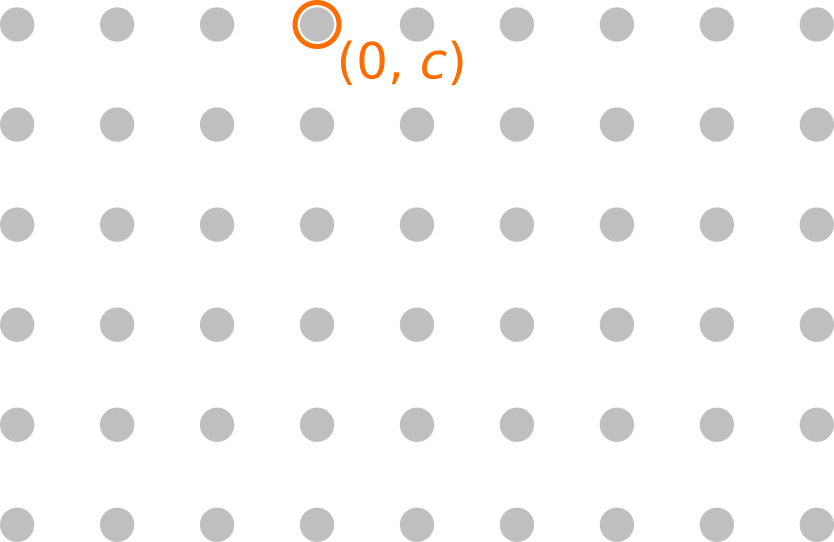
\includegraphics[scale=0.8]{square-f.png}
\end{itemize}

\end{frame}

\begin{frame}{Solution}

\begin{itemize}
    \item Algorithm 4 \\
        放置在 $(0, c)$ 的点在 $n \times m$ 网格图中影响的正方形个数 $f(n, m, c)$ \\ \\

        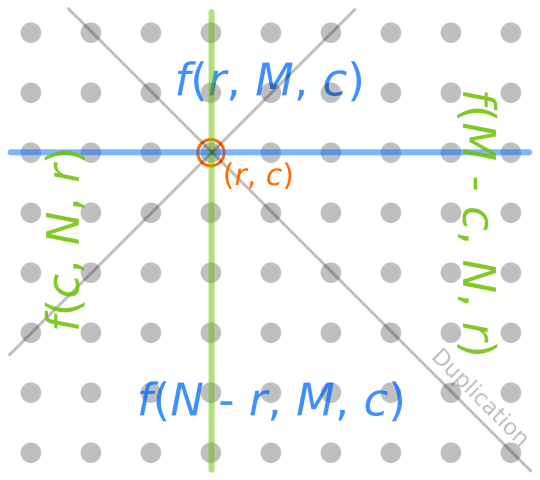
\includegraphics[scale=0.8]{square-aff1.png}

        \small{
        \begin{equation*}\begin{split}
            Aff_1(r, c) = &f(r, M, c) + f(N - r, M, c) + f(c, N, r) + f(M - c, N, r) \\
                & - (\min(r, c) + \min(r, M - c) + \min(N - r, c) + \min(N - r, M - c))
        \end{split}\end{equation*}}
\end{itemize}

\end{frame}

\begin{frame}{Solution}

\begin{itemize}
    \item Algorithm 4 \\
        放置在 $(0, c)$ 的点在 $n \times m$ 网格图中影响的正方形个数 $f(n, m, c)$

        $$
            f(n, m, c) = (\sum_{type = 0}^{\min(c, n)} \min(n - type + 1, m - c + 1)) - 1
        $$

        计算一个 $f$ 的时间复杂度为 $O(1)$,因此计算一个 $Aff_1$ 的时间复杂度为 $O(1)$。
\end{itemize}

\end{frame}

\begin{frame}{Solution}

\begin{itemize}
    \item Algorithm 4 \\
        $Aff_2$,$Aff_3$,$Aff_4$

        \pause 固定两个删除的点,检查另两个点是否被删除。$O(K^2 \cdot {\rm CheckState})$ \\
        \pause → 二分/\texttt{std::set} 可以把检查从 $O(K)$ 降为 $O(\log K)$ \\
        \pause 别忘了对角线 \\
         \\
        \pause 总时间复杂度:$O(\max(M, N) + K^2 \log K)$
        \begin{itemize}
            \item 预处理阶乘 \& 逆元:$O(\max(M, N))$
            \item 无坏点的情况 $F$:$O(1)$
            \item $Aff_1$:$O(1)$
            \item $Aff_{2 \dots 4}$:$O(K^2 \log K)$
        \end{itemize}
\end{itemize}

\end{frame}

%%%%%%%%%%%%%%%%%%%%%%%% Day 3 C %%%%%%%%%%%%%%%%%%%%%%%%

\begin{frame}{Problem 9. Mark}

THU 的 G 系有 $n$ 位同学和 $m$ 门必修课,分别编号 $0 \dots n - 1$,$0 \dots m - 1$。
一位同学在必修课 $i$ 上可以获得的分数是 $[1, u_i]$ 中的一个整数。

0 号同学 B 神在第 $i$ 门课上的排名是 $r_i$(i.e. 有且仅有 $r_i - 1$ 门同学
在这门课上分数\textbf{严格大于} B 神)。

如果每门课上 A 获得的成绩均\textbf{小于等于} B 获得的成绩,则称 A 被 B 碾压。
G 系一共有恰好 $k$ 位同学被 B 神碾压(不包括 B 神自己)。

求符合 B 神排名和碾压情况的情况数 $\mod 10^9 + 7$。两种情况不同当且仅当
有任意一位同学在任意一门课上获得的分数不同。同学之间是两两不同的。

\end{frame}

\begin{frame}{Problem 9. Mark}

\begin{tabularx}{\textwidth}{X|X|X|X} \hline
Case \# & $n$ & $m$ & $u_i$ \\ \hline \hline
1    & $\leq 3$   & $\leq 3$   & $\leq 4$    \\ \hline
2    & $\leq 3$   & $\leq 10$  & $\leq 100$  \\ \hline
3    & $\leq 3$   & $\leq 100$ & $\leq 10^9$ \\ \hline
4, 5 & $\leq 5$   & $\leq 100$ & $\leq 10^9$ \\ \hline
6, 7 & $\leq 50$  & $\leq 50$  & $\leq 50$   \\ \hline
8 \textasciitilde 10 & $\leq 100$ & $\leq 100$ & $\leq 10^9$ \\ \hline
\end{tabularx}

\end{frame}

\begin{frame}{Solution}

\begin{tabularx}{\textwidth}{X|X|X|X} \hline
Case \# & $n$ & $m$ & $u_i$ \\ \hline \hline
1    & $\leq 3$   & $\leq 3$   & $\leq 4$    \\ \hline
\end{tabularx}
\begin{itemize}
    \item Algorithm 1 \\
        枚举每个同学在每门课上的分数,并检查是否符合条件。

        时间复杂度 $O({u_{\max}}^{N \cdot M})$。
\end{itemize}

\end{frame}

\begin{frame}{Solution}

\begin{tabularx}{\textwidth}{X|X|X|X} \hline
Case \# & $n$ & $m$ & $u_i$ \\ \hline \hline
2    & $\leq 3$   & $\leq 10$  & $\leq 100$  \\ \hline
\end{tabularx}
\begin{itemize}
    \item Algorithm 2 \\
        由于必修课之间是独立的,枚举 B 神在这门课上的分数,并利用组合学公式计算情况数目。
        (本烧饼表示也不是很能理解 = =)

        时间复杂度 $O({u_{\max}}^N \cdot M)$。
\end{itemize}

\end{frame}

%%%%%%%%%%%%%%%%%%%%%%%% Day 4 B %%%%%%%%%%%%%%%%%%%%%%%%

\begin{frame}{Problem 11. Rand}

你的面前有 $n$ 个数排成一行,分别为 $a_1, a_2, \dots, a_n$。你打算在每相邻的两个
$a_i$ 和 $a_{i+1}$ 间都插入一个加号、减号或者乘号。那么一共有 $3^{n-1}$ 种可能的表达式。

进行 $Q$ 次修改操作,每次修改一个 $a_i$ 的值,之后输出所有可能的表达式的和 $\mod 10^9 + 7$。

\begin{tabularx}{\textwidth}{X|X} \hline
Case \# & $n, Q$ \\ \hline \hline
1, 2                 & $\leq 10$       \\ \hline
3 \textasciitilde 5  & $\leq 1\,000$   \\ \hline
6 \textasciitilde 10 & $\leq 100\,000$ \\ \hline
\end{tabularx}

\end{frame}

\begin{frame}{Solution}

\begin{tabularx}{\textwidth}{X|X} \hline
Case \# & $n, Q$ \\ \hline \hline
1, 2                 & $\leq 10$       \\ \hline
\end{tabularx}
\begin{itemize}
    \item Algorithm 1 \\
        枚举相邻两个数字之间的运算符,并计算表达式的值。

        时间复杂度 $O(3^{n-1} \cdot Q)$。
\end{itemize}

\end{frame}

\begin{frame}{Solution}

\begin{tabularx}{\textwidth}{X|X} \hline
Case \# & $n, Q$ \\ \hline \hline
3 \textasciitilde 5  & $\leq 1\,000$   \\ \hline
\end{tabularx}
\begin{itemize}
    \item Algorithm 2 \\
        \begin{align*}
            &a_1 \times a_2 \times \dots \times a_k + {\rm Bluh\ Bluh\ Bluh} \\
            &a_1 \times a_2 \times \dots \times a_k - {\rm Bluh\ Bluh\ Bluh}
        \end{align*}
        \pause
        $$
            Ans = \prod_{i = 1}^{n} a_i + \sum_{i = 1}^{n - 1} \left [\left (\prod_{j = 1}^i a_j \right ) \cdot 2 \cdot 3^{n - i - 1}\right ]
        $$

        直接计算即可,时间复杂度 $O(n \cdot Q)$。
\end{itemize}

\end{frame}

\begin{frame}{Solution}

\begin{tabularx}{\textwidth}{X|X} \hline
Case \# & $n, Q$ \\ \hline \hline
6 \textasciitilde 10 & $\leq 100\,000$ \\ \hline
\end{tabularx}
\begin{itemize}
    \item Algorithm 3 \\
        用线段树维护各种和啊积啊什么的……大家自己 YY 一下就好…… \\
        时间复杂度 $O(Q \log n)$。\\ \\
        \pause
        人群中钻出一个 CZR:“分块大法好 OwO” \\
        时间复杂度 $O(Q \sqrt n)$。\\
        \pause
        然而评测机比较慢。我得去喝杯 82 年的 Java 冷静冷静
\end{itemize}

\end{frame}

\end{document}
